\tikzset{%
  >=latex
}
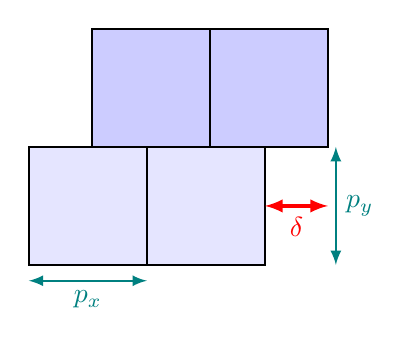
\begin{tikzpicture}[thick]
    % Define pixel size and offset
    \def\psize{1.5cm}
    \def\offset{0.8cm}

    % Draw bottom row (no offset)
    \draw[fill=blue!10] (0,0) rectangle (\psize,\psize);
    \draw[fill=blue!10] (\psize,0) rectangle (2*\psize,\psize);

    % Draw top row (with offset)
    \draw[fill=blue!20] (\offset,\psize) rectangle (\offset+\psize,2*\psize);
    \draw[fill=blue!20] (\offset+\psize,\psize) rectangle (\offset+2*\psize,2*\psize);

    % Draw horizontal offset arrow
    \draw[<->,very thick,red] (2*\psize,0.5*\psize) -- ++(\offset,0)
        node[midway,below] {$\delta$};

    % Label pixel dimensions
    \draw[<->,thick,teal] (2*\psize+\offset +0.1cm,0) -- ++(0,\psize)
        node[midway,right] {$p_y$};
    \draw[<->,thick,teal] (0,-0.2cm) -- ++(\psize,0)
        node[midway,below] {$p_x$};

\end{tikzpicture}
